\documentclass[]{article}

\usepackage{booktabs}
\usepackage{lipsum} 
\usepackage{graphicx}
\usepackage{tabularx}
\usepackage{float}
\usepackage{tikz}

\usepackage{amsmath}


\usepackage{geometry}
\geometry{a4paper, left=3cm, top=3cm, bottom=3cm, right=3cm}

\usepackage{caption}
\setlength{\abovecaptionskip}{10pt}

\usepackage{changepage}
\usepackage{pdfpages}
\usepackage{pdflscape}
\usepackage{threeparttable}


\usepackage{pgffor}

\usepackage{subcaption}

\usepackage{natbib}

\usepackage{subfiles}

\setlength{\abovedisplayskip}{10pt}
\setlength{\belowdisplayskip}{10pt}

% \pagestyle{empty}

\graphicspath{ {images/} }


\newcommand{\insertfigs}[2]{
    \begin{figure}[H]
        \caption{#1}
        \label{fig:#2}
        \foreach \name in \fields {
            \begin{subfigure}[p]{0.15\textheight}
                \centering
                \resizebox{0.8\textwidth}{!}{%
                    \includegraphics[width=\textwidth]{figures/#2/\name}
                }
                \caption{\name}
            \end{subfigure}\quad
        }
    \end{figure}
}

\newcommand{\insertfig}[2]{
    \begin{figure}[H]
        \caption{#1}
        \label{fig:#2}
        \includegraphics[width=\textwidth]{figures/#2}
    \end{figure}
}

\newcommand{\inserttable}[2]{
    \newgeometry{margin=2cm}
    \begin{landscape}
    \begin{table}[H]
        \caption{#1}
        \label{table:#2}
        \resizebox{\columnwidth}{!}{
            \input{tables/#2}
        }
    \end{table}
    \end{landscape}
    \restoregeometry
}

\newcommand{\tableref}[1]{
    \begin{center} 
        \textbf{[Table \ref{table:#1} about here]}
    \end{center}
}

\newcommand{\figref}[1]{
    \begin{center} 
        \textbf{[Fogure \ref{fig:#1} about here]}
    \end{center}
}

\newcommand*{\fields}{
    Artificial intelligence,
    Economics,
    Ethnic \string& cultural studies,
    Gender studies,
    Genetics \string& genomics,
    Geometry,
    Geophysics,
    Human resources \string& organizations,
    Immunology,
    International business,
    Language \string& linguistics,
    Material engineering,
    Neurology,
    Political science,
    Probability \string& statistics,
    Sociology
}

\newcommand{\insertfigsslides}[2]{
    \begin{adjustwidth}{-2em}{-2em}
        \begin{figure}[hbtp]
            % \caption{#1}
            \label{fig:#2}
            \foreach \name in \fields {
                \begin{subfigure}[p]{0.19\textheight}
                    \centering
                    \resizebox{0.75\textwidth}{!}{%
                        \includegraphics[width=\textwidth]{figures/#2/\name}
                    }
                    \caption{\name}
                \end{subfigure}\quad
            }
        \end{figure}
    \end{adjustwidth}
}

\newcommand{\insertfigslides}[1]{
    \includegraphics[keepaspectratio=true,width=\paperwidth, height=\paperheight]{figures/#1}
}

\newcommand*{\bivariates}{
    Density\_AvgDegree,
    Density\_Triangles,
    Density\_Louvain,
    Density\_Components,
    Density\_AvgClustering,
    Density\_Transitivity,
    Density\_Centralization,
    AvgClustering\_Centralization
}

\newcommand{\insertbivariatesslides}[1]{
    \begin{adjustwidth}{-2em}{-2em}
        \begin{figure}[hbtp]
            % \label{fig:#2}
            \foreach \name in \bivariates {
                \begin{subfigure}[p]{0.25\textheight}
                    \centering
                    \resizebox{0.75\textwidth}{!}{%
                        \includegraphics[width=\textwidth]{figures/all_bivariate/\name}
                    }
                    \caption{\name}
                \end{subfigure}\quad
            }
        \end{figure}
    \end{adjustwidth}
}



% \tikzstyle{vertex}=[draw,fill=black!15,circle,minimum size=18pt,inner sep=0pt]

\begin{document}

% High -> Low -> High Centrlization (cycles)
% Number of communities

% Likert scale (High, Medium Low) on each dimension

% There are n patterns along which fields develop

    \pagenumbering{gobble}

    \subfile{sections/title_page}

    \tableofcontents

    \newpage

    \listoffigures
    \listoftables
    
    % \cleardoublepage

    % \pagenumbering{arabic}

    % 
\begin{abstract}
    This paper examines the structure and dynamics of science across 16 fields by analyzing both 
    bibliographic and semantic networks. The study finds that there are few structural differences
    between the fields, indicating that the underlying structure of scientific knowledge is 
    relatively uniform. The analysis reveals that there are common patterns of co-citation and term 
    co-occurrence, highlighting the interconnected nature of scientific research.
\end{abstract}

    % \section{Introduction}

    % 
\begin{itemize}

	\item "Form of scientific \textbf{organization} [...] \textbf{mode of organization}" \citep[158-160]{collins1994}

	\item "\textbf{What is distinctive} about the social organization of the disciplines that we now take as natural science, and do the social disciplines have (or can they acquire) the \textbf{conditions that make possible that kind of organization}?" \citep[156]{collins1994}

	\item What sets appart "\textbf{high-consensus rapid-discovery}" from "\textbf{social}" science and "\textbf{humanities}"? \citep[158]{collins1994}

	\item "Hard" v. "Soft" sciences

\end{itemize}



















% \only<1>{
	
% 	\framesubtitle{Origin of the debate}

% 	Structure \string& dynamics of science
	
% 	\begin{itemize}
		
% 		\item \cite{popper2002}: Methods \string& falsification
		
% 		\item "Recurrent debates about whether one or another of the contemporary social sciences is really a science [...] will cease to be a source of concern not when a definition is found, but when the groups that now doubt their own status achieve \textbf{consensus} about their past and present accomplishments" \citep[160-161]{kuhn2012}
		
% 	\end{itemize}
% }

% \only<2>{

% 	\framesubtitle{Questions}

% 	\begin{itemize}

% 	\item How do the characteristics of natural sciences compare to those of social sciences and humanities in terms of cumulativeness, and what structural factors contribute to these differences?

% 	\item Which fields, if any, can be characterized as "high-consensus, rapid-discovery" \citep{collins1994} and how do these fields differ from others in terms of structure?

% 	\item How do the structural features of different scientific fields vary, and what factors contribute to these differences?

% 	\end{itemize}
% 	\framesubtitle{}

% 	Do different scientific fields differ in their structural features?

% 	Previous litterature:

% 	\begin{itemize}

% 	\item Single field \citep{cahlik2006,yeung2017,qin2020}

% 	\item Temporality \citep{callon2005,beam2014}

% 	\item Qualitative \citep{popper2002,kuhn2012,collins1994,silverstein1991}

% 	\end{itemize}
% }

% \only<3> {
	
% 	\framesubtitle{Function \string& Dynamics}

% 	\fontsize{10}{10}\selectfont
% 	\begin{multicols}{2}
% 	\begin{itemize}
% 		\item “Communities” \citep{kuhn2012}
% 		\item “Tribes” \citep{trowler2001}
% 		\item “Invisible colleges” \citep{desollaprice1966, crane1972, paisley1972}
% 		\item “Teams” \citep{wuchty2007}
% 		\item “Social-intellectual movements” \citep{frickel2005} 
% 		\item “Bandwagons” \citep{shannon1956}
% 		\item “Actor-networks” \citep{latour1988} 
% 		\item “Theory groups” \citep{mullins1973}
% 		\item "Programmes” \citep{lakatos1968,merton1972}
% 		\item “Schools" \citep{radnitzky1971,tiryakian1979}
% 		\item “Specialty” \citep{wray2005}
% 		\item “Parallel processing units” \citep{kornfeld1981}
% 		\item “Invisible brain [regions]” \citep{segev2016}
% 		\item "Complex system" \citep{boulding1956}
% 		\item “Referee system” \citep{zuckerman1971}	
% 	\end{itemize}
% 	\end{multicols}
% }

    % \section{Theory}

    % 
\subsection{Revolutionary Science}

\cite{kuhn2012} posits that scientific knowledge advances through periods of incremental progress punctuated by abrupt, revolutionary changes in understanding. According to Kuhn, during normal science, scientists work within an accepted paradigm, which is a set of assumptions, concepts, and methods that define a scientific discipline at a given time. Scientists in a paradigm share a common language, a set of beliefs, and a set of practices that enable them to conduct research and generate new knowledge within the paradigm.

However, as anomalies and inconsistencies between what the models predict and what is observed accumulate within the paradigm, scientists may begin to question its validity, and a crisis may emerge. During this crisis, scientists may propose new theories and methods that challenge the existing paradigm. If a new theory is accepted, it may eventually replace the old paradigm, leading to a scientific revolution.

\subsection{Fractal Science}

\citeauthor{abbott2001}'s \citeyearpar{abbott2001} fractal division of disciplines is a model that suggests that any discipline can be divided into smaller sub-disciplines, which in turn can be further divided into smaller sub-sub-disciplines, and so on, creating a fractal-like structure.

Figure \ref{fig:fractal_distinctions} (p. 14)

\begin{figure}[H]
	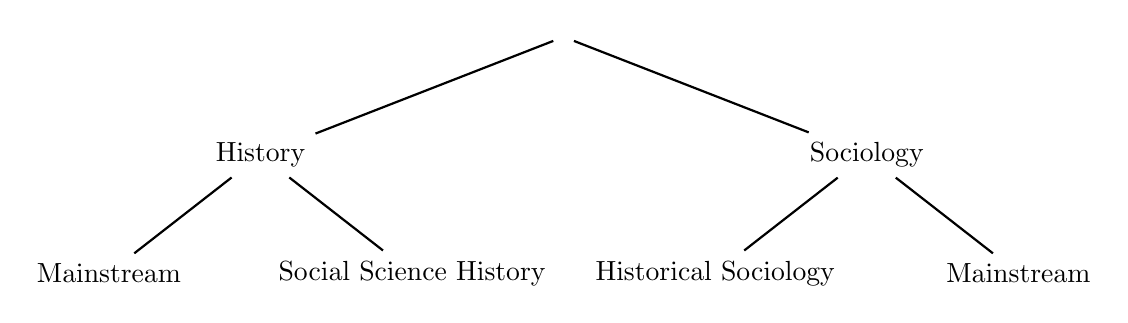
\begin{tikzpicture}[thick,level/.style={sibling distance=77mm/#1}]
	\node [] (r) {}
	  child {
	    node [] (a) {History}
	    child {
	      node [] {Mainstream}
	    }
	    child {
	      node [] {Social Science History}
	    }
	  }
	  child {
	    node [] {Sociology}
	    child {
	      node [] {Historical Sociology}
	    }
	    child {
	      node [] {Mainstream}
	    }
	  };
	\end{tikzpicture}
	\caption{Fractal Distinctions} 
	\label{fig:fractal_distinctions}
\end{figure}

\subsection{High Consensus, Rapid Discovery Science}

\cite{collins1994} posits that achieving high levels of consensus and rapid scientific discovery in science research relies on the use of research technologies and techniques that generate consistent, observable, and reliable data, resulting in a high degree of reproducibility. As a result, conflict and disagreement are limited to the frontiers of research. 

The natural sciences have experienced high levels of consensus and rapid scientific discovery since the post-scientific revolution of the 1600s, but this has not been solely due to empiricism, mathematization, measurement precision, or the experimental method that existed before this era. Instead, the distinguishing feature of this time period has been the creation of research technologies that facilitate the production of new data and observations.

The social sciences face obstacles not solely due to a lack of common ideas, as Kuhn suggests, but also from a dearth of technologies that produce consistent data and results: "The most glaring lack within social science is a self-generating lineage of research technologies" (p. 165).

\subsection{Attention in Science}

The "Law of Small Numbers" is a concept first introduced by \cite{collins1998}, which is based on the idea of a "limited attention space" which sets an upper bound on the possible number of subfields in a field. This concept has been further developed by other researchers, with Price (1986) suggesting that the number of items that can be held in attention is around five, while Collins himself revised this number to seven in 1994. In other words, the "Law of Small Numbers" is analogous to a carrying capacity.

A binomial distribution can be used to describe the number of groups competing for attention in situations where there are two possible outcomes for each group (i.e. success or failure in acquiring the resource). The binomial distribution can be used to calculate the probability of a given number of groups successfully acquiring the resources. For example, if there are 10 groups competing for a finite number of resources, the binomial distribution can be used to calculate the probability of each possible number of groups (from 0 to 10) successfully acquiring the resources. I expect to observe a binomial distribution with a mode of anywhere between 1 and 7 for the number of subfields in a field, but most likely between 5 and 7.

\subsection{Phases of Science}

\cite{mullins1973} proposed a model for the development of scientific fields that incorporates elements from both the "invisible college" \citep{desollaprice1966, crane1969, crane1972, paisley1972} and "scientific revolutions" \citep{kuhn2012}. According to Mullins, the development of scientific fields is determined by the interactions and competition between different "theory groups", which are networks of scientists who share similar ideas and interests.

Mullin's model consists of four stages, which are as follows:

\begin{enumerate}

\item Normal: In the normal stage of theory group development, the communication network among researchers is loosely coupled, meaning that there is only a weak connection between the different researchers within the group. This stage is characterized by low clustering and density, and individual researchers are largely focused on solving specific problems within the field. This stage is similar to what Kuhn (1962) referred to as the "puzzle-solving" or "paradigmatic" phase of scientific development, in which researchers are largely focused on applying established theories and methods to the study of specific phenomena. In this phase, there is little attention to or interest in alternative paradigms or theories, and the focus is on making incremental advances within the existing framework.

\item Network: In the network stage of theory group development, the patterns of communication among researchers begin to change due to the emergence of one or more influential ideas or theories that attract the attention of multiple researchers. This leads to a shift in the focus of the group and the development of a consensus among its members, which allows for the creation of an alternative paradigm or approach to the problem they are studying. As the group becomes more focused and cohesive, communication within the group increases, while communication with external researchers or other groups declines. In this phase, the group's success in advancing their ideas and theories is crucial for maintaining its growth and attracting new members.

\item Cluster: The third stage of theory group development, known as the cluster phase, is characterized by the emergence of a power-law distribution of communication ties among researchers. In this phase, clusters of researchers typically form around the most productive or influential members of the group, who can often be found in one or a few institutions. This creates a positive feedback loop, where the ideas and theories of the most productive researchers are reinforced and strengthened by the input and support of the other members of the cluster. This can lead to the institutionalization of the group and its ideas, as the cluster becomes increasingly recognized and respected within the broader field. As the group's ideas and theories evolve, they may also begin to diverge from the established concepts and theories of the parent discipline, reflecting the group's growing focus and specialization. According to Mullin (1973), the degree of divergence from the parent field is a function of the group's size and isolation, with larger and more isolated groups being more likely to develop their own distinct paradigms and theories. 

At this point, the group can take one of two possible trajectories, depending on the parent discipline's reaction to the group's ideas. If the parent discipline rejects or ignores the group's ideas, the group may become isolated and continue to develop their ideas independently, remaining in the cluster stage. This is often referred to as a "revolutionary" trajectory, as the group is effectively challenging the existing paradigms and theories of the parent discipline. On the other hand, if the parent discipline adopts or diffuses the group's ideas, the group may become integrated into the broader field and recognized as an "elite" group. In this case, the group's ideas may become mainstream and widely accepted within the parent discipline.

\item Speciality: The final stage of theory group development, known as the specialty phase, is only reached by "elite" groups whose ideas are adopted and diffused by the parent discipline. In this phase, the group's members may begin to scatter and move to different institutions or locations, weakening the connections within the group and enabling the diffusion of their ideas to a wider audience. This process of scattering and diffusion can lead to the routinization and institutionalization of the group's ideas, as they become integrated into the broader field of knowledge and accepted as a new paradigm or approach. Over time, the dense network of communication within the group may begin to loosen again, returning to the more loosely-coupled, normal pattern of communication seen in the earlier stages of theory group development.

\end{enumerate}

The transition between the different phases of theory group development is not guaranteed, and groups may fail or die off before reaching the later stages. The success of a group and its ability to advance through the different phases is contingent on a number of factors, including its ability to grow and attract new members at a faster rate than alternative groups. This in turn is dependent on factors such as the group's apparent success in advancing their ideas, the presence of strong intellectual leaders within the group, the support and recognition of the broader community, the availability of research centers and materials to support the group's work, and the output of textbooks and other materials that can help to promote and disseminate the group's ideas.





    % \section{Methods}

    % 
\subsection{Data}

Top 5 journals from \href{https://scholar.google.com/citations?view_op=top_venues}{Google Scholar Top Publication}

\begin{figure}
    \centering
    \begin{minipage}[t]{0.4\textwidth}\centering
    	\begin{itemize}
    		\item Artificial Intelligence
			\item Economics
			\item Ethnic \& Cultural Studies
			\item Gender Studies
			\item Genetics \& Genomics
			\item Geometry
			\item Geophysics
			\item Human Resources \& Organizations
    	\end{itemize}
    \end{minipage}\hfill
    \begin{minipage}[t]{0.4\textwidth}\centering
    	\begin{itemize}
    		\item Immunology
			\item International Business
			\item Language \& Linguistics
			\item Material Engineering
			\item Neurology
			\item Political Science
			\item Probability \& Statistics
			\item Sociology
		\end{itemize}
    \end{minipage}
\end{figure}

\subsection{Networks}


\subsection{Citation}

A citation network represented as a directed unweighted graph, with nodes representing individual 
documents and edges indicating a citation from one document to another.

\begin{figure}[H]
    \centering
    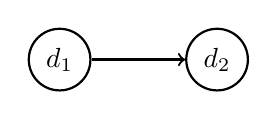
\begin{tikzpicture}[node distance=2cm, thick, main/.style = {draw, circle}]
        \node[main] (1) [] {$d_1$};
        \node[main] (2) [right of=1] {$d_2$};
        \draw[->] (1) -- (2);
    \end{tikzpicture}
    \caption{Citation} \label{fig:citation}
\end{figure}

Figure \ref{fig:citation} depicts a citation diad in which document $d_1$ cites document $d_2$.

\subsection{Co-Citation}

A co-citation network represented as an undirected weighted graph, with nodes corresponding to 
individual documents and edge weights representing the frequency with which two documents are 
co-cited.

\begin{figure}[H]
    \centering
    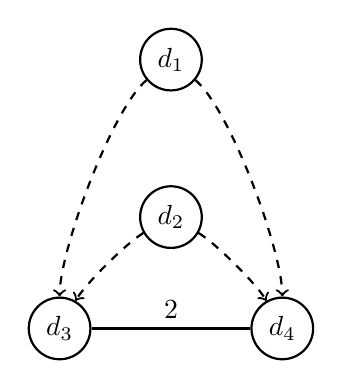
\begin{tikzpicture}[node distance=2cm, thick, main/.style = {draw, circle}]
        \node[main] (1) [] {$d_1$};
        \node[main] (2) [below of=1] {$d_2$};
        \node[main] (3) [below left of=2] {$d_3$};
        \node[main] (4) [below right of=2] {$d_4$};
        \draw[->] (1) to [out=220, in=90, looseness=0.5] (3) [dashed] node {};
        \draw[->] (1) to [out=320, in=90, looseness=0.5] (4) [dashed] node {};
        \draw[->] (2) to [out=210, in=60, looseness=0.5] (3) [dashed] node {};
        \draw[->] (2) to [out=330, in=120, looseness=0.5] (4) [dashed] node {};
        \draw[] (3) -- node[midway, above] {2} (4);
    \end{tikzpicture}
    \caption{Co-Citation} \label{fig:co_citation}
\end{figure}

As shown in Figure \ref{fig:co_citation}, the edge weight of 2 between documents $d_3$ and $d_4$ reflects 
the fact that they are co-cited by two documents, $d_1$ and $d_2$.

\subsection{Co-Occurrence}

A co-occurrence network represented as an undirected weighted graph, with nodes representing 
individual terms and edge weights indicating the frequency with which two terms co-occur within a 
document.

\begin{figure}[H]
    \centering
    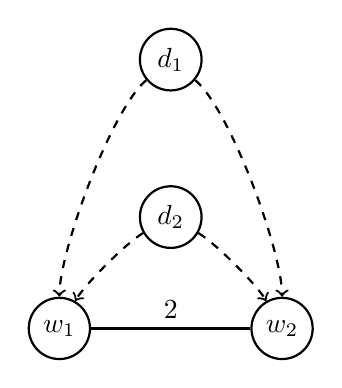
\begin{tikzpicture}[node distance=2cm, thick, main/.style = {draw, circle}]
        \node[main] (1) [] {$d_1$};
        \node[main] (2) [below of=1] {$d_2$};
        \node[main] (3) [below left of=2] {$w_1$};
        \node[main] (4) [below right of=2] {$w_2$};
        \draw[->] (1) to [out=220, in=90, looseness=0.5] (3) [dashed] node {};
        \draw[->] (1) to [out=320, in=90, looseness=0.5] (4) [dashed] node {};
        \draw[->] (2) to [out=210, in=60, looseness=0.5] (3) [dashed] node {};
        \draw[->] (2) to [out=330, in=120, looseness=0.5] (4) [dashed] node {};
        \draw[] (3) -- node[midway, above] {2} (4);
    \end{tikzpicture}
    \caption{Co-Occurrence} \label{fig:co_occurrence}
\end{figure}

As shown in Figure \ref{fig:co_occurrence}, the edge weight of 2 between terms $w_3$ and $w_4$ 
reflects the fact that they co-occur in both documents, $d_1$ and $d_2$.

% \insertimage{citation_graphs}{Discipline Citation Graphs}

\subsection{ERGMs}

The probability of observing a particular network structure is modeled as a function of various network statistics or features.

In their general form, ERGMs are written as \citep{hunter2008}:

$$
P(Y=y) = \frac{exp[\beta_1 s_1(g) + \beta_2 s_2(g) + ... + \beta_p s_p(g)]}{\sum\limits_{g'} exp[\beta_1 s_1(g') + \beta_2 s_2(g') + ... + \beta_p s_p(g')]}
$$

\begin{itemize}
    \item Y is the random variable for the state of the network (with realization y)
    \item $s_k(g)$ is a $k$th model statistics (ERGM term) for the network $g$
    \item $\beta_k$ is the coefficients the sufficient statistic $k$
\end{itemize}

% \break

% Denominator:

% \begin{itemize}
% 	\item Undirected: $2^{(n(n-1)/2)}$ 
% 	\item Directed: $2^{(n(n-1))}$
% \end{itemize}

% Because of this, Markov Chain Monte Carlo Maximum Likelihood Estimation (MCMC MLE) is used to estimate the denominator. It samples from the space of all possible networks producing a representative sample and estimate of the true denominator. 

% \break

% The ergm equation can be re-written in terms of change statistics. The log-odds of a tie $ij$ is:

% $$
% logit(Y_{ij} = 1 | y_{ij}^c) = \theta' \delta(y_{ij})
% $$

% Where:
% \begin{itemize}
% 	\item $y_{ij}^c$ is the complement of $y_{ij}$, i.e. all dyads in the network other than $y_{ij}$
% 	\item $\theta'$ is the vector of coefficients for the sufficient statistics
% 	\item $y_{ij}^+$ as the same network as $y$ except that $y_{ij} = 1$
% 	\item $y_{ij}^-$ as the same network as $y$ except that $y_{ij} = 0$
% 	\item $\delta(y_{ij})$ is given by $g(y_{ij}^+) - g(y_{ij}^-)$ which measures how the sufficient 
% 	statistic $g(y)$ changes if the $(i, j)$th edge is toggled on or off.
% \end{itemize}

\break

To obtain the probability of observing an edge, the expit (or inverse logit) of $\beta$ is taken:

$$
P(e) = \frac{\exp(\beta)}{(1 + exp(\beta))}
$$

Quantifying the importance of a structure in the network formation process


















\subsection{Measurements}

\only<1>{
Following \citet{jiao2017} I define the network measurments and the expected direction of their effect
}

\only<2>{
    \framesubtitle{Density effect (Edges)}

    Density refers to the proportion of connections in a social network relative to the total possible connections.

    This is interpreted as the intercept of the model. The entry of the `density` matrix $M_{ij}$ indicates how the presence of that edge changes the number of edges in the graph, holding the rest of the network constant. It a matrix of ones - with the upper right triangle masked in the case of undirected networks.
}

\only<3>{
    \framesubtitle{Small-World effect (Triangles)}

    Set of three documents or concepts who are mutually connected, are a common feature of social networks and are thought to play an important role in social cohesion and network structure \citep{kossinets2006, newman2018}.
}

\only<4>{
    \framesubtitle{Silo effect (Components)}

    silos refer to isolated areas of research or knowledge that are not well connected to other areas or fields limit the flow of information and influence within the network
    Hyper specialization of field of knowledge
    Talk to one another but never talk to nodes outside their primary group
}

\only<5>{
    \framesubtitle{Closure effect (Transitivity)}

    A triad is a group of three nodes in a graph. A triad can either be open or closed. An open triad is a group of three nodes that are connected by two edges (Figure \ref{fig:open_triad}), while a closed triad is a group of three nodes that are connected by three edges (Figure \ref{fig:closed_triad}). 

    \begin{figure}[H]
        \centering
        \begin{subfigure}[t]{0.4\textwidth}
            \centering
            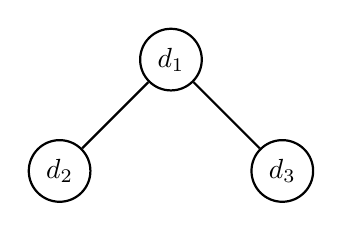
\begin{tikzpicture}[node distance=2cm, thick, main/.style = {draw, circle}]
                \node[main] (1) [] {$d_1$};
                \node[main] (2) [below left of=1] {$d_2$};
                \node[main] (3) [below right of=1] {$d_3$};
                \draw[] (1) to (2);
                \draw[] (1) to (3);
            \end{tikzpicture}
            \caption{Open Triad} 
            \label{fig:open_triad}
         \end{subfigure}
            ~
         \begin{subfigure}[t]{0.4\textwidth}
            \centering
            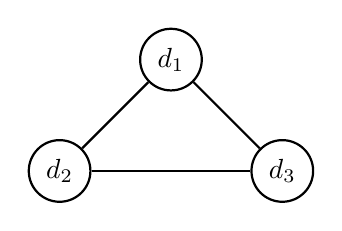
\begin{tikzpicture}[node distance=2cm, thick, main/.style = {draw, circle}]
                \node[main] (1) [] {$d_1$};
                \node[main] (2) [below left of=1] {$d_2$};
                \node[main] (3) [below right of=1] {$d_3$};
                \draw[] (1) to (2);
                \draw[] (1) to (3);
                \draw[] (2) to (3);
            \end{tikzpicture}
            \caption{Closed Triad} 
            \label{fig:closed_triad}
         \end{subfigure}
         \caption{Triads}
    \end{figure}

    Transitivity is defined as the ratio of the number of closed triads in the graph to the number of open triads in the graph.

    $$
    T = \frac{3t_c}{t_o}
    $$

    Where $t_c$ is the number of closed triads and $t_o$ is the number of open triads.
}

\only<6>{
    \framesubtitle{Clique effect (Cliques)}

    Tendecy for there to be parts of the graph where multiple nodes all co-occur more than by random change

    If I discuss 
    A all other concepts in the clique it belongs to.
    highly related to each other distinct topical or functional units within the network

    This build on triangles (which are a clique) but captures more information 

    It asks whether triangles overlap to form larger structurees rather than just isolated (random) triangles

    Densly connected always connected
}

\only<7>{
    \framesubtitle{Popularity effect ($k$-star)}

    The popularity effects in most classes were not obvious, which meant the degree (the total number of actors selecting an individual) of individuals in the class networks had little difference.

    \begin{figure}[H]
        \centering
        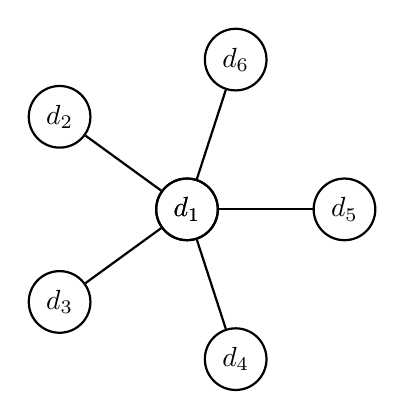
\begin{tikzpicture}[node distance=2cm, thick, main/.style = {draw, circle}]
            \node[main] (1) at (360:0mm) (center) {$d_1$};
            \node[main] (1) [] {$d_1$};
            \foreach \n in {2,...,6}{
                \node[main] at ({\n*360/5}:2cm) (n\n) {$d_\n$};
                \draw (center)--(n\n);
            }
        \end{tikzpicture}
        \caption{Star} \label{fig:k_star}
    \end{figure}

    What we mean by a strong k star effect
    Control for 9 stars in order to determine if 10 star is significant
    10 star is a bunch of 9 stars
}

\only<8>{
    \framesubtitle{Mediating effect (betweenness centrality)}

    Nodes with high betweenness centrality in this type of network may represent important bridge terms or pivot terms that connect different topics or themes within the corpus of documents. The betweenness centrality $c_b$ of node $n$ is given by:

    $$
    c_b(i) = \sum_{j \ne k} \frac{\sigma_{jk}(i)}{\sigma_{jk}}
    $$

    Where $\sigma_{ij}$ is the total number of shortest paths from node $i$ to node $j$ and $\sigma_{ij}(n)$ is the number of those paths that pass through node $n$. In other words, it is the proportion of all shortest paths between nodes $i$ and $j$ that pass through node $n$. The average betweenness centrality over all nodes of the network is taken as another network statistic. 

    Indicates good integration but maybe structural fragility (if central nodes are removed, speperate components)
}

\only<9>{
    \framesubtitle{Community effect (Louvain)}

    The Louvain community detection method consists of two main steps. Initially, each node is assigned to a separate community. Then, for each node, the algorithm attempts to optimize the modularity of the network by evaluating the potential gain in modularity achieved by moving the node to each of its neighboring communities. If no gain is achieved, the node remains in its original community.

    In the second step, a new network is constructed where each node represents a community from the previous step. The edges between the new nodes are weighted by the sum of the weights of the edges between the nodes in the corresponding communities in the original network. The Louvain method is then applied to this new network, and the process is repeated until no further improvement in modularity can be achieved.

    Modularity is a measure of the degree of segregation of a network into communities. It is calculated 
    as the difference between the fraction of edges within a given group and the expected fraction of 
    edges if they were randomly distributed in the network. The change in modularity $\Delta Q$ achieved 
    by moving the node to each of its neighboring communities is measured as

    $$
    Q = \frac{1}{2m}\sum_{i,j}[A_{ij} - \frac{k_ik_j}{2m}]\delta(c_i,c_j)
    $$

    where:
    \begin{itemize}
        \item $Q$ is the modularity index
        \item $m$ is the total number of edges in the network
        \item $A_{ij}$ is the weight of the edge between nodes $i$ and $j$
        \item $k_i$ and $k_j$ are the degrees of nodes $i$ and $j$, respectively
        \item $c_i$ and $c_j$ are the community assignments of nodes $i$ and $j$
        \item $\delta(c_i,c_j)$ is the Kronecker delta, which is equal to 1 if nodes $i$ and $j$ are in the same community and 0 otherwise.
    \end{itemize}
}



    % \section{Data}

    % Top 5 journals from \href{https://scholar.google.com/citations?view_op=top_venues}{Google Scholar Top Publication}

\begin{figure}
    \centering
    \begin{minipage}[t]{0.4\textwidth}\centering
    	\begin{itemize}
    		\item Artificial Intelligence
			\item Economics
			\item Ethnic \& Cultural Studies
			\item Gender Studies
			\item Genetics \& Genomics
			\item Geometry
			\item Geophysics
			\item Human Resources \& Organizations
    	\end{itemize}
    \end{minipage}\hfill
    \begin{minipage}[t]{0.4\textwidth}\centering
    	\begin{itemize}
    		\item Immunology
			\item International Business
			\item Language \& Linguistics
			\item Material Engineering
			\item Neurology
			\item Political Science
			\item Probability \& Statistics
			\item Sociology
		\end{itemize}
    \end{minipage}
\end{figure}

    % \section{ERGMs}

    % The probability of observing a particular network structure is modeled as a function of various network statistics or features.

In their general form, ERGMs are written as \citep{hunter2008}:

$$
P(Y=y) = \frac{exp[\beta_1 s_1(g) + \beta_2 s_2(g) + ... + \beta_p s_p(g)]}{\sum\limits_{g'} exp[\beta_1 s_1(g') + \beta_2 s_2(g') + ... + \beta_p s_p(g')]}
$$

\begin{itemize}
    \item Y is the random variable for the state of the network (with realization y)
    \item $s_k(g)$ is a $k$th model statistics (ERGM term) for the network $g$
    \item $\beta_k$ is the coefficients the sufficient statistic $k$
\end{itemize}

% \break

% Denominator:

% \begin{itemize}
% 	\item Undirected: $2^{(n(n-1)/2)}$ 
% 	\item Directed: $2^{(n(n-1))}$
% \end{itemize}

% Because of this, Markov Chain Monte Carlo Maximum Likelihood Estimation (MCMC MLE) is used to estimate the denominator. It samples from the space of all possible networks producing a representative sample and estimate of the true denominator. 

% \break

% The ergm equation can be re-written in terms of change statistics. The log-odds of a tie $ij$ is:

% $$
% logit(Y_{ij} = 1 | y_{ij}^c) = \theta' \delta(y_{ij})
% $$

% Where:
% \begin{itemize}
% 	\item $y_{ij}^c$ is the complement of $y_{ij}$, i.e. all dyads in the network other than $y_{ij}$
% 	\item $\theta'$ is the vector of coefficients for the sufficient statistics
% 	\item $y_{ij}^+$ as the same network as $y$ except that $y_{ij} = 1$
% 	\item $y_{ij}^-$ as the same network as $y$ except that $y_{ij} = 0$
% 	\item $\delta(y_{ij})$ is given by $g(y_{ij}^+) - g(y_{ij}^-)$ which measures how the sufficient 
% 	statistic $g(y)$ changes if the $(i, j)$th edge is toggled on or off.
% \end{itemize}

\break

To obtain the probability of observing an edge, the expit (or inverse logit) of $\beta$ is taken:

$$
P(e) = \frac{\exp(\beta)}{(1 + exp(\beta))}
$$

Quantifying the importance of a structure in the network formation process


















    % \section{Measurements}

    % \only<1>{
Following \citet{jiao2017} I define the network measurments and the expected direction of their effect
}

\only<2>{
    \framesubtitle{Density effect (Edges)}

    Density refers to the proportion of connections in a social network relative to the total possible connections.

    This is interpreted as the intercept of the model. The entry of the `density` matrix $M_{ij}$ indicates how the presence of that edge changes the number of edges in the graph, holding the rest of the network constant. It a matrix of ones - with the upper right triangle masked in the case of undirected networks.
}

\only<3>{
    \framesubtitle{Small-World effect (Triangles)}

    Set of three documents or concepts who are mutually connected, are a common feature of social networks and are thought to play an important role in social cohesion and network structure \citep{kossinets2006, newman2018}.
}

\only<4>{
    \framesubtitle{Silo effect (Components)}

    silos refer to isolated areas of research or knowledge that are not well connected to other areas or fields limit the flow of information and influence within the network
    Hyper specialization of field of knowledge
    Talk to one another but never talk to nodes outside their primary group
}

\only<5>{
    \framesubtitle{Closure effect (Transitivity)}

    A triad is a group of three nodes in a graph. A triad can either be open or closed. An open triad is a group of three nodes that are connected by two edges (Figure \ref{fig:open_triad}), while a closed triad is a group of three nodes that are connected by three edges (Figure \ref{fig:closed_triad}). 

    \begin{figure}[H]
        \centering
        \begin{subfigure}[t]{0.4\textwidth}
            \centering
            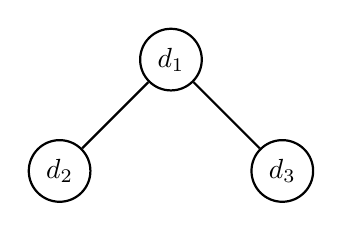
\begin{tikzpicture}[node distance=2cm, thick, main/.style = {draw, circle}]
                \node[main] (1) [] {$d_1$};
                \node[main] (2) [below left of=1] {$d_2$};
                \node[main] (3) [below right of=1] {$d_3$};
                \draw[] (1) to (2);
                \draw[] (1) to (3);
            \end{tikzpicture}
            \caption{Open Triad} 
            \label{fig:open_triad}
         \end{subfigure}
            ~
         \begin{subfigure}[t]{0.4\textwidth}
            \centering
            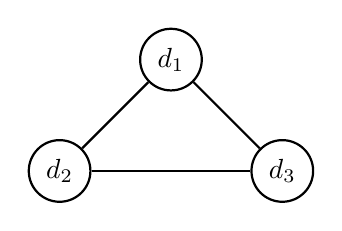
\begin{tikzpicture}[node distance=2cm, thick, main/.style = {draw, circle}]
                \node[main] (1) [] {$d_1$};
                \node[main] (2) [below left of=1] {$d_2$};
                \node[main] (3) [below right of=1] {$d_3$};
                \draw[] (1) to (2);
                \draw[] (1) to (3);
                \draw[] (2) to (3);
            \end{tikzpicture}
            \caption{Closed Triad} 
            \label{fig:closed_triad}
         \end{subfigure}
         \caption{Triads}
    \end{figure}

    Transitivity is defined as the ratio of the number of closed triads in the graph to the number of open triads in the graph.

    $$
    T = \frac{3t_c}{t_o}
    $$

    Where $t_c$ is the number of closed triads and $t_o$ is the number of open triads.
}

\only<6>{
    \framesubtitle{Clique effect (Cliques)}

    Tendecy for there to be parts of the graph where multiple nodes all co-occur more than by random change

    If I discuss 
    A all other concepts in the clique it belongs to.
    highly related to each other distinct topical or functional units within the network

    This build on triangles (which are a clique) but captures more information 

    It asks whether triangles overlap to form larger structurees rather than just isolated (random) triangles

    Densly connected always connected
}

\only<7>{
    \framesubtitle{Popularity effect ($k$-star)}

    The popularity effects in most classes were not obvious, which meant the degree (the total number of actors selecting an individual) of individuals in the class networks had little difference.

    \begin{figure}[H]
        \centering
        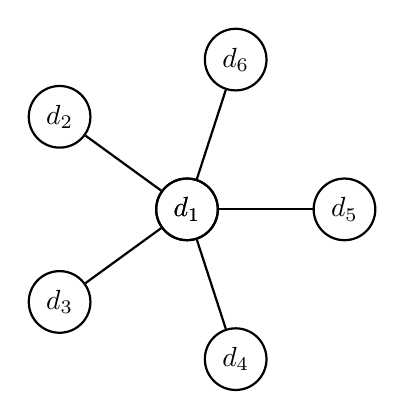
\begin{tikzpicture}[node distance=2cm, thick, main/.style = {draw, circle}]
            \node[main] (1) at (360:0mm) (center) {$d_1$};
            \node[main] (1) [] {$d_1$};
            \foreach \n in {2,...,6}{
                \node[main] at ({\n*360/5}:2cm) (n\n) {$d_\n$};
                \draw (center)--(n\n);
            }
        \end{tikzpicture}
        \caption{Star} \label{fig:k_star}
    \end{figure}

    What we mean by a strong k star effect
    Control for 9 stars in order to determine if 10 star is significant
    10 star is a bunch of 9 stars
}

\only<8>{
    \framesubtitle{Mediating effect (betweenness centrality)}

    Nodes with high betweenness centrality in this type of network may represent important bridge terms or pivot terms that connect different topics or themes within the corpus of documents. The betweenness centrality $c_b$ of node $n$ is given by:

    $$
    c_b(i) = \sum_{j \ne k} \frac{\sigma_{jk}(i)}{\sigma_{jk}}
    $$

    Where $\sigma_{ij}$ is the total number of shortest paths from node $i$ to node $j$ and $\sigma_{ij}(n)$ is the number of those paths that pass through node $n$. In other words, it is the proportion of all shortest paths between nodes $i$ and $j$ that pass through node $n$. The average betweenness centrality over all nodes of the network is taken as another network statistic. 

    Indicates good integration but maybe structural fragility (if central nodes are removed, speperate components)
}

\only<9>{
    \framesubtitle{Community effect (Louvain)}

    The Louvain community detection method consists of two main steps. Initially, each node is assigned to a separate community. Then, for each node, the algorithm attempts to optimize the modularity of the network by evaluating the potential gain in modularity achieved by moving the node to each of its neighboring communities. If no gain is achieved, the node remains in its original community.

    In the second step, a new network is constructed where each node represents a community from the previous step. The edges between the new nodes are weighted by the sum of the weights of the edges between the nodes in the corresponding communities in the original network. The Louvain method is then applied to this new network, and the process is repeated until no further improvement in modularity can be achieved.

    Modularity is a measure of the degree of segregation of a network into communities. It is calculated 
    as the difference between the fraction of edges within a given group and the expected fraction of 
    edges if they were randomly distributed in the network. The change in modularity $\Delta Q$ achieved 
    by moving the node to each of its neighboring communities is measured as

    $$
    Q = \frac{1}{2m}\sum_{i,j}[A_{ij} - \frac{k_ik_j}{2m}]\delta(c_i,c_j)
    $$

    where:
    \begin{itemize}
        \item $Q$ is the modularity index
        \item $m$ is the total number of edges in the network
        \item $A_{ij}$ is the weight of the edge between nodes $i$ and $j$
        \item $k_i$ and $k_j$ are the degrees of nodes $i$ and $j$, respectively
        \item $c_i$ and $c_j$ are the community assignments of nodes $i$ and $j$
        \item $\delta(c_i,c_j)$ is the Kronecker delta, which is equal to 1 if nodes $i$ and $j$ are in the same community and 0 otherwise.
    \end{itemize}
}

    % \section{Descriptive Statistics}

    % 
Bibliometric networks exhibit the following characteristics \citep{holme2002}:

\begin{itemize}
\item They are large and sparse graphs, meaning that only a small fraction of all possible edges 
actually exist \citep{watts1998,newman2003,jackson2010}
\item The average geodesic (shortest path) length grows logarithmically \citep{leskovec2007}
\item The degree distribution approximately follows a power law decay \citep{barabasi1999}
\item They exhivit a high degree of clustering \citep{newman2003,kretschmer2004}
\end{itemize}
    
    % \section{Results}

    % 

\inserttable{ergm}{ERGM Results}

\subsection{Density Effect (Edges)}

Both co-citation and co-occurrence graphs are found to be sparse for every discipline, which is 
indicated by the negative and significant coefficients. A sparse network is characterized by a 
relatively low proportion of connections between individuals in comparison to the total number of 
potential connections that can exist within the network.

\subsection{Small-World effect (Triangles)}

As suggested by prior research, the social networks under investigation demonstrate a higher 
prevalence of triangles than what would be expected by random chance. Triangles, which represent a 
set of three documents or concepts who are mutually connected, are a common feature of social networks and are 
thought to play an important role in social cohesion and network structure 
\citep{kossinets2006, newman2018}. The observed excess of 
triangles in the current study is consistent with previous findings on the presence of triadic 
closure in social networks, where nodes tend to form connections with the neighbors of their 
neighbors \citep{burt2000}.

All coefficients that are statistically significant for triangles exhibit a positive sign, which 
suggests that triangles are present in the social network under investigation at a rate higher than 
that which would be expected by chance alone.



    % \newpage

    % \bibliographystyle{utils/ajs}
    % \bibliography{sections/bibliography}

    % \newpage

    
    %%%%%%%%%%%%%%%%%%%%%%%%%%%%%%%%%%%%%%%%%%%%%%%%%%%%%%
    %%% Citation
    %%%%%%%%%%%%%%%%%%%%%%%%%%%%%%%%%%%%%%%%%%%%%%%%%%%%%%

    % \newpage
    
    % \insertfig{Citation Graphs}{citation_graphs}

    % \newpage

    % \insertfig{Citation Temporal Cumulative Distribution}{citation_temp_cum_dist}

    % \newpage

    % \insertfig{Co-Citation Node Distance Distribution}{co_citation_node_distance_dist}

    % \newpage

    % \insertfig{Citation Temporal DAG Longest Patg}{citation_temp_dag_longest_path}

    % \newpage
    
    % \insertfig{Citation Degree Distribution}{citation_deg_dist}

    % \newpage

    % \inserttable{Citation Descriptive Statistics}{citation_desc_stats}

    % \newpage

    % \inserttable{Citation Reference Dates}{citation_ref_dates}

    % \newpage

    % \insertfig{Citation Reference Dates Distribution}{citation_ref_dates}

    %%%%%%%%%%%%%%%%%%%%%%%%%%%%%%%%%%%%%%%%%%%%%%%%%%%%%%
    %%% Co-Citation
    %%%%%%%%%%%%%%%%%%%%%%%%%%%%%%%%%%%%%%%%%%%%%%%%%%%%%%

    % \newpage

    % \insertfig{Co-Citation Graphs\\$(e = 50)$}{co_citation_graphs}
    
    % \newpage

    % \inserttable{Co-Citation Descriptive Statistics}{co_citation_desc_stats}

    % \newpage

    % \insertfig{Co-Citation Degree Distribution}{co_citation_deg_dist}

    \newpage

    \inserttable{Co-Citation ERGM Model}{co_citation_ergm_model}

    %%%%%%%%%%%%%%%%%%%%%%%%%%%%%%%%%%%%%%%%%%%%%%%%%%%%%%
    %%% Co-Occurrence
    %%%%%%%%%%%%%%%%%%%%%%%%%%%%%%%%%%%%%%%%%%%%%%%%%%%%%%

    % \newpage

    % \insertfig{Co-Occurrence Graphs\\$(e = 100)$}{co_occurrence_graphs}

    % \newpage

    % \inserttable{Co-Occurrence Descriptive Statistics}{co_occurrence_desc_stats}

    % \newpage

    % \insertfig{Co-Occurrence Degree Distribution\\$(w > 1)$}{co_occurrence_degree_dist}

    % \newpage

    % \insertfig{Co-Occurrence Node Distance Distribution}{co_occurrence_node_distance_dist}

    % \newpage

    \inserttable{Co-Occurrence ERGM Model}{co_occurrence_ergm_model}


\end{document}